%\documentclass{report}
%\usepackage{fullpage}
%%\usepackage[top=1in, bottom=1in]{geometry}
%\usepackage{amsfonts}
%%for math symbols, Ex: \mathbb{N}
%\def\Definition{what does something mean}
%\usepackage{graphicx}
%\usepackage[hidelinks]{hyperref}
%\usepackage{pdfpages}
%\usepackage{float}
%\begin{document}

\chapter{Introduction}

Jet noise has been the subject of intensive research since the dawn of jet engine. Most of the research in the early decades had been focussed on subsonic noise \cite{lighthill}. But, as the technology improved and our ambitions widened, more  resources have been dedicated to understand noise generated at high speeds. Surprisingly, It has not been as difficult as expected to garner information from supersonic noise mechanisms owing to their characteristic nature \cite{tam1}. 

\section{Supersonic noise mechanism}

Supersonic noise comprises of mainly three components (fig \ref{fig:noise}).\\ 

\begin{figure}[H]
	\centering
	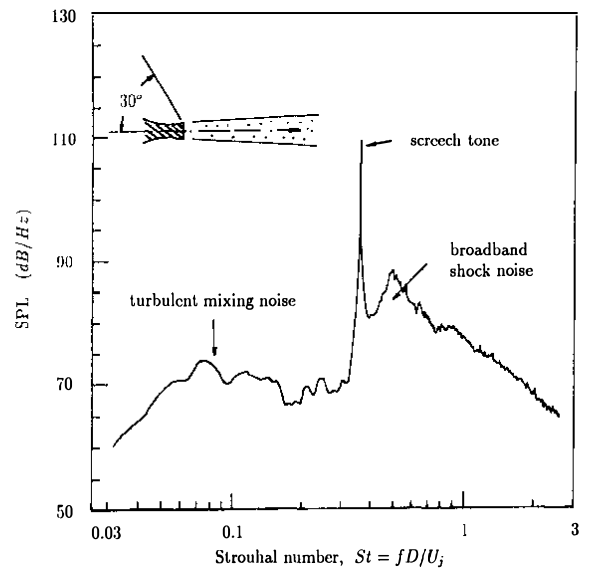
\includegraphics[width=3in]{images/noise.png}
	\caption{Supersonic jet noise spectrum, Seiner 1984, as published in Tam\cite{tam3}}
	\label{fig:noise}
\end{figure} 

\noindent
Turbulent mixing noise is predominantly due to large turbulent structures moving at supersonic speeds leading to phenomenon like mach wave radiation. Although fine turbulent structures also contribute to what is considered background noise, they are not as dominant as they are in subsonic flows. This noise is high at lower angles to jet and decreases as we move upstream.\\
\par\par

\noindent
Broadband shock noise (BBSN) is due to the interaction between turbulent structures and quasi periodic shock cells in the flow. Perfectly expanded flow is ideally not expected to encounter this noise since there should be no shocks/expansions to be 
reflected by mixing layer. Since the shocks cells are very well defined, the directivity and strength of this noise is much easier to formulate analytically unlike subsonic noise. This noise dominates at higher angles upstream\\ 
\par

\noindent
Screeching noise, easiest to notice in the fig \ref{fig:noise}, is considered to be a special case of broadband shock noise. When the turbulent structures interact with shock cell, acoustic waves are generated. These waves, of certain frequency band, travel outside jet and interact with lip region which inturn affects the generation of turbulent structures completing a feedback loop. It is important to note that the peaks of broadband shock noise and turbulent mixing noise vary with the observation angle (angle with respect to jet axis, 0 being along the jet). But the frequency of screech tone is same for all observation points. More interestingly, its frequency  always forms lower bound of broadband shock peak and they tend to merge as the angle increases. Infact, if we use angle $180^0$ in the formula to calculate the peak frequency of BBSN, we get the frequency value of screech tone \cite{tam1}.\\
\par 
As we have seen, frequency analysis of pressure data goes a long way to explain noise mechanisms. This report is to use similar techniques to study various scales of velocity and TKE data from steady PIV. Since we don't have time data, wavelength analysis has been done and compared with analytical shock cell information. 

%\end{document}